\section{Baseline (2017): encoder--decoder Transformer}

\begin{frame}{The 2017 Transformer}
  \centering
  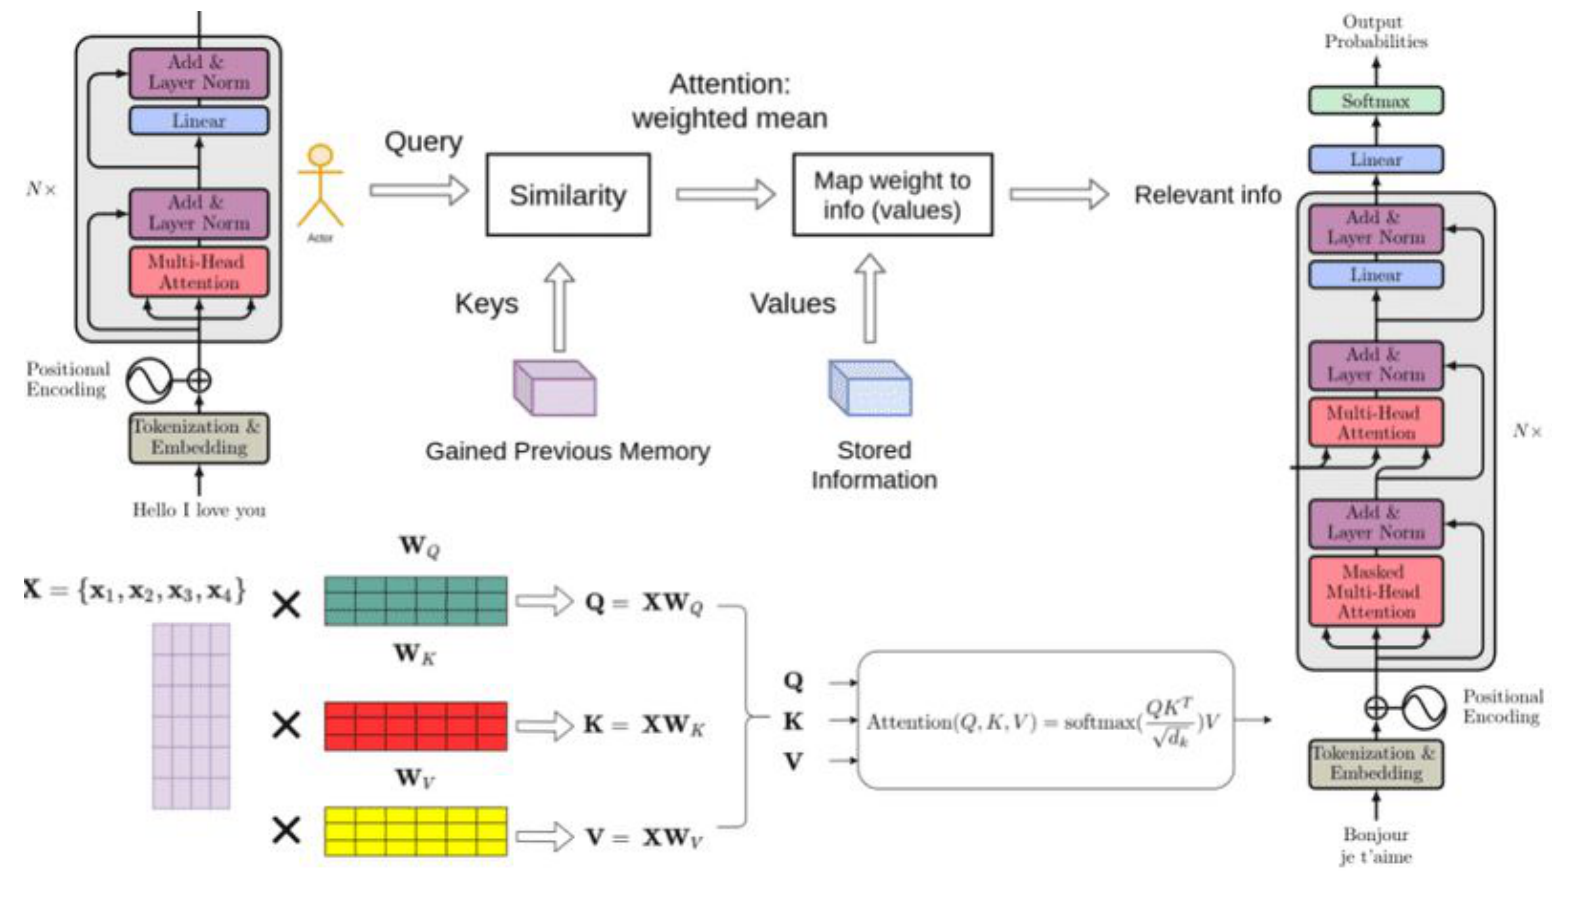
\includegraphics[width=0.5\paperwidth,height=0.95\paperheight,keepaspectratio]{images/introduction-to-transformers/transformer_attention_overview_qkv_architecture.png}
\end{frame}

\begin{frame}{Why the Transformer?}
  \begin{itemize}
    \item The original 2017 Transformer was designed to address key limitations of Recurrent Neural Networks (RNNs) and Long Short-Term Memory (LSTM) units:
      \begin{itemize}
        \item Lack of parallelization
        \item Vanishing gradient problem inherent in sequential processing
      \end{itemize}
    \item Replaced recurrence with self-attention to allow all tokens in a sequence to be processed simultaneously during training\footnote{See Vaswani et al., ``Attention is All You Need,'' 2017.}
    \item Enabled significant reductions in wall-clock time needed for model convergence
  \end{itemize}
\end{frame}

\begin{frame}{The 2017 Building Blocks (Recap)}
  \begin{columns}
    \begin{column}{0.53\textwidth}
      \begin{itemize}
        \item[$\blacktriangleright$] Tokenization and input embeddings
        \item[$\blacktriangleright$] Sinusoidal position encodings
        \item[$\blacktriangleright$] Self-attention over Query, Key, Value
        \item[$\blacktriangleright$] Multi-head attention
        \item[$\blacktriangleright$] Feed-forward blocks with Add \& Norm
        \item[$\blacktriangleright$] Encoder stack, decoder stack, masked and cross-attention
      \end{itemize}
\end{column}
    \begin{column}{0.47\textwidth}
      \centering
      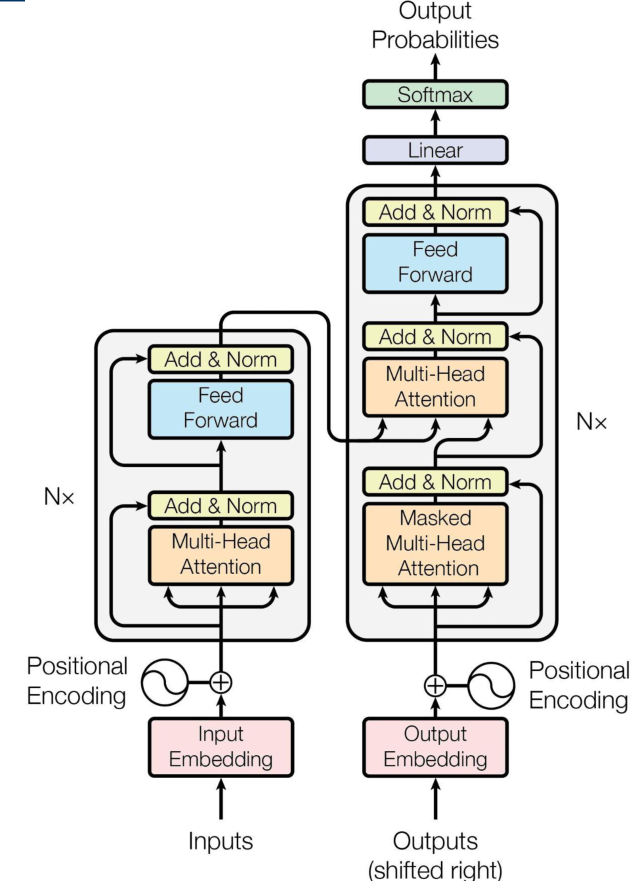
\includegraphics[width=0.9\linewidth,height=0.9\textheight,keepaspectratio]{images/introduction-to-transformers/transformer_vaswani_encoder_decoder_diagram.png}
    \end{column}
  \end{columns}
\end{frame}

\begin{frame}{Scaled Dot-Product and Multi-Head Attention (Recap)}
  \textbf{Scaled dot-product attention:}
  \begin{align*}
    \text{Attention}(Q, K, V) = \mathrm{softmax}\left(\frac{QK^T}{\sqrt{d_k}}\right)V
  \end{align*}

  \vspace{0.5em}
  \textbf{Multi-head attention:}
  \[
    \mathrm{MultiHead}(Q, K, V) = \mathrm{Concat}(\text{head}_1, \ldots, \text{head}_h) W^O,
    \quad
    \text{head}_i = \mathrm{Attention}(Q W_i^Q, K W_i^K, V W_i^V)
  \]

  \vspace{0.5em}
  \begin{itemize}
    \item[$\blacktriangleright$] Every token attends to every other token: quadratic cost in sequence length.
    \item[$\blacktriangleright$] In 2017 every head carries its own full $K$ and $V$ projections; MQA and GQA later relax this.
  \end{itemize}
\end{frame}
